\begin{figure}[H]
  \centering
  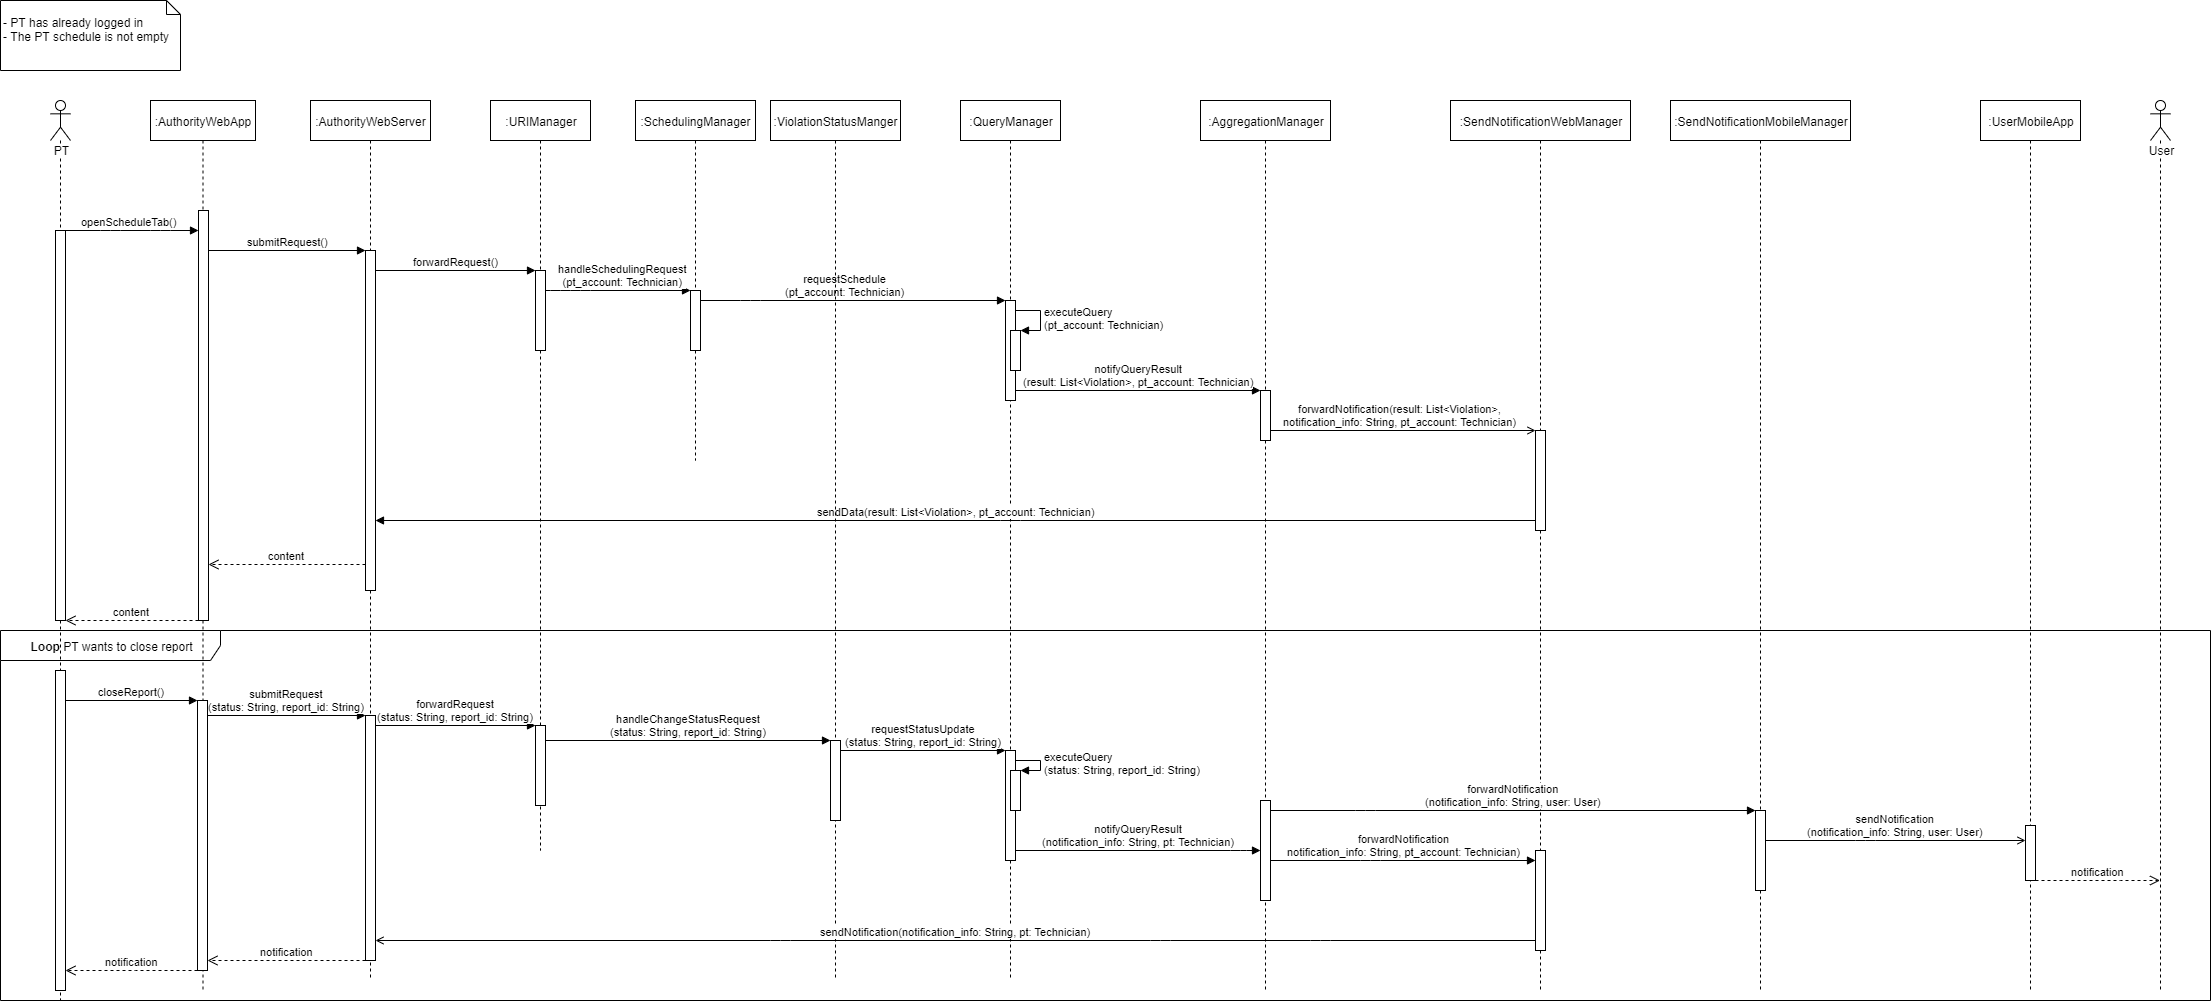
\includegraphics[width=1\textwidth]{Images/UML_diagrams/Sequence_Diagrams/Watch_schedule_sd.png}
  \caption{Watch assigned schedule sequence diagram}
  \label{fig:watch_schedule_sd}
\end{figure}
This sequence diagram is related to consulting the schedule assigned to a PT and optionally to the closing of a report. Once the PT opens his schedule tab a request to retrieve his plan is submitted. The request that arrives to the URIManager is forwarded to the SchedulingManager that will request to the QueryManager to perform a query to retrieve the schedule associated to that PT account. The result is as usual forwarded to the AggregationManager that will pack it in a suitable format and forward it back to the web app via the SendNotificationWebManager. If the technician choose to close a particular report (i.e. setting its status to closed) he can submit a request for such change. When this request reaches the URIManager component it will be forwarded to the ViolationStatusManager that will request to the QueryManager to make an update query to change the status of the specified report. When the update is done, a notification is sent both to the technician and to the user that submitted the report via their appropriate notification component. 
